\documentclass[a4paper]{article}

\usepackage[utf8]{inputenc}  
\usepackage[francais]{babel}  
\usepackage[top=2cm, bottom=2cm, left=2cm, right=2cm]{geometry}
\usepackage{graphicx}
\usepackage{algorithmic}
\usepackage{algorithm}

\renewcommand{\algorithmicrequire}{\textbf{Input:}}
\renewcommand{\algorithmicensure}{\textbf{Output:}}

\begin{document}

\begin{titlepage}
	~ 
	\vfill
	\begin{center}
		\begin{Huge}
			Projet Grammaire et langage : \\ Dossier de rendu\\
		\end{Huge}
	\vfill
		\textbf{Hexanôme 4211 :} 
			\\Sandra \bsc{Mondain}, Elisa \bsc{Abidh}, 
			\\Gaël \bsc{Motte}, Armand \bsc{Rossius}, 
			\\Nicolas \bsc{Silva}, Julien \bsc{Levesy}\\
	\vfill
	\end{center}
	\vfill
\end{titlepage}

\newpage
\tableofcontents
\newpage

\section{Structure de Données}
ici sont a coller tous les chémas concernant les différentes structures de données.

\subsection{Xml}
\begin{figure}[H]
	\begin{center}
	% l b r t
		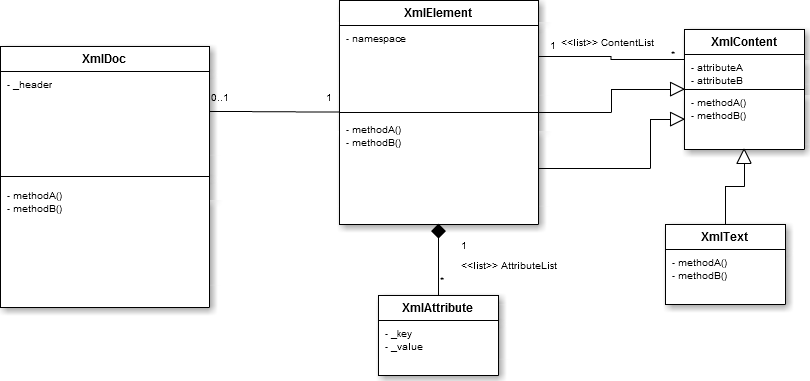
\includegraphics[scale=0.5]{IMG/XmlStructures.png}
		\caption{Structure de données pour un document Xml}
	\end{center}
\end{figure}

\subsection{Dtd}
\begin{figure}[H]
	\begin{center}
	% l b r t
		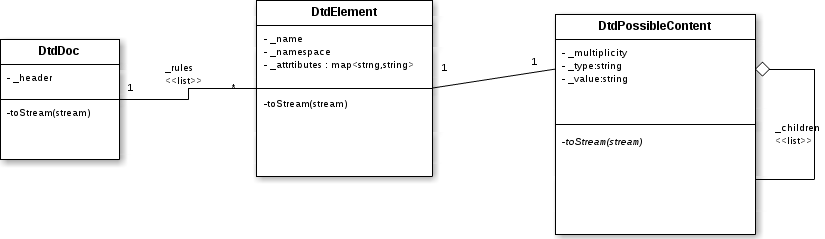
\includegraphics[scale=0.5]{IMG/DtdStructures.png}
		\caption{Structure de données pour un document Dtd}
	\end{center}
\end{figure}



\section{Algorithmes}

\subsection*{Introduction}
\paragraph{Visitor}
La totalité de notre conception repose en grande partie sur l'utilisation du \textit{design pattern visitor}. Le concept de ce design pattern repose sur le double dispatch qui permet de réduire les dépendance des algorithmes vis à vis des structures de données.\\


\subsection{Algorithme générale de validation}
La validation se fait en suivant le principe d'un parcours d'arbre en profondeur. Chaque noeud du document xml ne sera donc validé que si ses fils ont été validé avant.



%%%%%%%%%%%%%%%%%%%%%%%%%%%%%%%%%%%%%%%%%%%%%%%%%%%%%%%%%%%%%%%%%%%%%%%%%%%%%%%%%%%%%%%
\begin{algorithm}
\caption{Validation d'un Document Xml}
\label{ValidateXmlDoc}
\begin{algorithmic}
\REQUIRE xmlDoc \COMMENT{Document à valider}
\IF {xmlDoc.Racine est valide} 
       \RETURN vrai
\ELSE
        \RETURN faux
\ENDIF 
\end{algorithmic}
\end{algorithm}
%%%%%%%%%%%%%%%%%%%%%%%%%%%%%%%%%%%%%%%%%%%%%%%%%%%%%%%%%%%%%%%%%%%%%%%%%%%%%%%%%%%%%%%
\begin{algorithm}
\caption{Validation d'un Element Xml}
\label{ValidateXmlElement}
\begin{algorithmic}
\REQUIRE xmlElement \COMMENT{Element à valider}
\STATE dtdDef $\Leftarrow$ DefinitionDtd(Element)
\IF {dtdDef n'existe pas} 
       \RETURN faux
\ELSE

	\FORALL[On descend dans l'arbre]{fils de xmlElement}
		\STATE visiter fils
		\IF{fils invalid}
			\RETURN faux
		\ENDIF
	\ENDFOR
	
	\STATE validation des attributs\COMMENT{cf Algorithm~\ref{CheckAttributes}}
	\IF{les attributs ne sont pas valides}
		\RETURN faux
	\ENDIF
	\STATE validation du contenu de l'élément\COMMENT{cf Algorithm~\ref{CheckContent}}
	\IF{\NOT Contenu est valide (element)}
		\RETURN faux
	\ENDIF

        \RETURN vrai
\ENDIF 
\end{algorithmic}
\end{algorithm}
%%%%%%%%%%%%%%%%%%%%%%%%%%%%%%%%%%%%%%%%%%%%%%%%%%%%%%%%%%%%%%%%%%%%%%%%%%%%%%%%%%%%%%%
\begin{algorithm}
\caption{Validation des attributs d'un Element Xml}
\label{CheckAttributes}
\begin{algorithmic}
\REQUIRE xmlElement \COMMENT{Element dont les attributs sont à valider}
\STATE dtdDef $\Leftarrow$ DefinitionDtd(Element)
\IF[cas superflu dans l'utilisation normale]{dtdDef n'existe pas} 
       \RETURN faux
\ELSE
	\FORALL[On parcours tous les attributs]{Attribut de xmlElement}
		\IF{attributs non défini dans dtdDef}
			\RETURN faux
		\ENDIF
	\ENDFOR
	\RETURN vrai
\ENDIF 
\end{algorithmic}
\end{algorithm}
%%%%%%%%%%%%%%%%%%%%%%%%%%%%%%%%%%%%%%%%%%%%%%%%%%%%%%%%%%%%%%%%%%%%%%%%%%%%%%%%%%%%%%%
~\\
Le déroulement de l'algorithme de validation sémantique des contenus fils du document Xml
est très commenté dans le fichier source XmlValidatorVisitor.cpp (méthode \textit{XmlValidatorVisitor.visitContentRecurse}). En raison de la taille de l'algorithme ainsi que des efforts mis en places pour le commenter, la présentation sous forme algorithmique s'est révélée plus difficile à lire que le listing original. Aussi le fonctionnement de l'algorithme est détaillé directement dans le code source.
~\\
\begin{algorithm}
\caption{Validation du contenu immédiat d'un Element Xml}
\label{CheckContent}
\begin{algorithmic}
\REQUIRE xmlIter \COMMENT{Itérateur vers un contenu fils de l'élément xml }
\REQUIRE xmlIterEnd \COMMENT{Itérateur de fin des contenus fils de l'élément xml }
\REQUIRE possibleContent \COMMENT{noeud de l'arbre des contenus possibles de l'élément xml }
\STATE dtdDef $\Leftarrow$ DefinitionDtd(Element)
\IF{possibleContent.type $=$ SEQUENCE} 
  \IF{possibleContent.multiplicity $=$ NORMAL}
    \STATE traitement particulier (cf. XmlValidatorVisitor.cpp)
  \ELSIF{possibleContent.multiplicity $=$ STAR}
    \STATE traitement particulier (cf. XmlValidatorVisitor.cpp)
  \ELSIF{possibleContent.multiplicity $=$ QMARK}
    \STATE traitement particulier (cf. XmlValidatorVisitor.cpp)
  \ELSIF{possibleContent.multiplicity $=$ PLUS}
    \STATE traitement particulier (cf. XmlValidatorVisitor.cpp)
  \ENDIF
\ELSIF{possibleContent.type $=$ CHOICE}
  \IF{possibleContent.multiplicity $=$ NORMAL}
    \STATE traitement particulier (cf. XmlValidatorVisitor.cpp)
  \ELSIF{possibleContent.multiplicity $=$ STAR}
    \STATE traitement particulier (cf. XmlValidatorVisitor.cpp)
  \ELSIF{possibleContent.multiplicity $=$ QMARK}
    \STATE traitement particulier (cf. XmlValidatorVisitor.cpp)
  \ELSIF{possibleContent.multiplicity $=$ PLUS}
    \STATE traitement particulier (cf. XmlValidatorVisitor.cpp)
  \ENDIF
\ELSIF{possibleContent.type $=$ ELEMENT}
	\IF{possibleContent.multiplicity $=$ NORMAL}
    \STATE traitement particulier (cf. XmlValidatorVisitor.cpp)
  \ELSIF{possibleContent.multiplicity $=$ STAR}
    \STATE traitement particulier (cf. XmlValidatorVisitor.cpp)
  \ELSIF{possibleContent.multiplicity $=$ QMARK}
    \STATE traitement particulier (cf. XmlValidatorVisitor.cpp)
  \ELSIF{possibleContent.multiplicity $=$ PLUS}
    \STATE traitement particulier (cf. XmlValidatorVisitor.cpp)
  \ENDIF
\ENDIF 
\end{algorithmic}
\end{algorithm}





\end{document}
